\chapter{Struktura systemu}
\label{cha:struktura-systemu}

System OSK-Manager został zaprojektowany jako aplikacja webowa z podziałem na kilka logicznych warstw. Taki podział ułatwia rozwój systemu, testowanie poszczególnych modułów oraz oddzielenie logiki prezentacji od logiki biznesowej i dostępu do danych.

\section{Ogólna architektura}
\label{sec:ogolna-architektura}

Architektura systemu składa się z następujących elementów:
\begin{itemize}
    \item warstwy frontendowej, odpowiedzialnej za interfejs użytkownika,
    \item warstwy BFF w aplikacji Nuxt, odpowiedzialnej za pośredniczenie w komunikacji z API,
    \item backendu Express, odpowiedzialnego za realizację logiki biznesowej,
    \item warstwy usług i walidacji, odpowiedzialnej za reguły domenowe,
    \item warstwy dostępu do danych opartej o Prisma,
    \item relacyjnej bazy danych PostgreSQL.
\end{itemize}

Użytkownik korzysta z aplikacji przez przeglądarkę internetową. Interfejs wysyła żądania do tras serwerowych Nuxt albo bezpośrednio do API, zależnie od konfiguracji. Backend odbiera żądanie, sprawdza sesję użytkownika, waliduje dane wejściowe, wykonuje logikę biznesową w odpowiednim serwisie i zapisuje lub odczytuje dane z bazy.

\section{Warstwa frontendowa}
\label{sec:warstwa-frontendowa}

Frontend odpowiada za prezentację danych oraz obsługę interakcji użytkownika. W projekcie zastosowano strukturę opartą na stronach, komponentach, kompozycjach i typach. Strony odpowiadają konkretnym widokom aplikacji, na przykład listom kursantów, harmonogramowi, szczegółom instruktora lub panelowi konta. Komponenty wielokrotnego użytku obsługują formularze, tabele, kalendarze, dialogi i elementy nawigacyjne.

Istotną częścią frontendu są kompozycje, które wydzielają logikę pobierania danych, filtrowania, paginacji oraz obsługi formularzy poza same komponenty widoku. Dzięki temu kod interfejsu pozostaje czytelniejszy, a operacje takie jak pobranie listy pojazdów, zapis kursanta albo odświeżenie harmonogramu mogą być używane w spójny sposób w wielu miejscach aplikacji.

\section{Warstwa BFF}
\label{sec:warstwa-bff}

W aplikacji frontendowej znajduje się warstwa BFF, czyli Backend for Frontend. Jest ona realizowana przez trasy serwerowe Nuxt. Jej zadaniem jest dopasowanie komunikacji do potrzeb interfejsu użytkownika oraz ukrycie części szczegółów backendu przed przeglądarką.

Warstwa BFF obsługuje między innymi przekazywanie żądań do backendu, normalizację odpowiedzi, walidację parametrów żądań oraz tryb mock dla wybranych danych w środowisku demonstracyjnym. Dzięki temu frontend może korzystać z jednolitego sposobu komunikacji, nawet jeżeli część danych pochodzi z backendu, a część z adapterów testowych.

\section{Warstwa backendowa}
\label{sec:warstwa-backendowa}

Backend został podzielony na trasy, kontrolery, serwisy, schematy walidacji oraz moduły pomocnicze. Trasy określają adresy endpointów HTTP. Kontrolery odpowiadają za odbiór żądania, wywołanie odpowiedniej usługi i zwrócenie odpowiedzi. Serwisy zawierają właściwą logikę biznesową, na przykład sprawdzanie dostępności instruktora, zapis lekcji, obsługę płatności lub walidację przynależności danych do konkretnego OSK.

W systemie można wyróżnić następujące główne moduły backendu:
\begin{itemize}
    \item moduł autoryzacji i profilu użytkownika,
    \item moduł ośrodków szkolenia kierowców,
    \item moduł kursantów,
    \item moduł instruktorów,
    \item moduł pojazdów,
    \item moduł typów kursów i kursów,
    \item moduł lekcji,
    \item moduł wydarzeń instruktorskich,
    \item moduł harmonogramu,
    \item moduł ocen lekcji,
    \item moduł płatności i planów płatności.
\end{itemize}

\section{Opis bazy danych}
\label{sec:opis-bazy-danych}

Baza danych systemu została zaprojektowana jako relacyjny model danych. Centralnym elementem modelu jest użytkownik, który może pełnić jedną z ról: kursanta, instruktora, managera lub administratora. Dane wspólne użytkownika przechowywane są w encji użytkownika, natomiast dane specyficzne dla roli są wydzielone do profilu kursanta lub profilu instruktora.

Ośrodek szkolenia kierowców grupuje kursantów, instruktorów, pojazdy, kursy oraz ustawienia organizacyjne. Dzięki temu system może obsługiwać wiele szkół jazdy i jednocześnie kontrolować, czy użytkownik wykonuje operacje wyłącznie na danych powiązanych z właściwym ośrodkiem.

Kurs jest powiązany z ośrodkiem, typem kursu oraz uczestnikami. Uczestnictwo kursanta w kursie opisuje osobna encja, która pozwala przechowywać status udziału kursanta. Lekcja jest przypisana do kursu, kursanta i instruktora, a w przypadku lekcji praktycznej może być dodatkowo powiązana z pojazdem. Taki model pozwala sprawdzać, czy lekcja została zaplanowana dla właściwego kursanta, właściwego kursu i właściwej szkoły.

Pojazdy są przypisane do ośrodka i posiadają dane takie jak nazwa, numer rejestracyjny, marka, model, rok produkcji, przebieg, zdjęcie oraz status dostępności. Pojazd może być używany w lekcjach praktycznych oraz wydarzeniach instruktorskich. System przechowuje również informacje o domyślnym pojeździe szkoły.

Dostępność instruktorów jest modelowana przez kilka powiązanych encji. Domyślne godziny pracy określają typowy tygodniowy grafik instruktora. Wyjątki dzienne pozwalają zmienić godziny pracy w konkretnym dniu. Blokady czasu opisują przerwy, spotkania lub inne zajęcia, natomiast urlopy określają dłuższe okresy niedostępności. Na podstawie tych danych oraz już istniejących lekcji system może wyliczać wolne terminy.

Wydarzenia instruktorskie opisują zajęcia typu jazda lub teoria. Mogą posiadać uczestników, powiązany kurs, pojazd, pojemność i status. Dzięki temu system obsługuje nie tylko pojedyncze lekcje, lecz także zajęcia grupowe lub inne zdarzenia widoczne w harmonogramie instruktora.

Rozliczenia kursu opisują plany płatności oraz płatności. Plan płatności przechowuje łączną kwotę, walutę, typ płatności i liczbę rat, natomiast płatność opisuje konkretną kwotę, termin płatności, datę opłacenia, status i metodę płatności.

Oceny lekcji przechowywane są w osobnej encji powiązanej z lekcją, kursantem oraz instruktorem. Dzięki temu kursant może ocenić zakończoną lekcję praktyczną, a manager lub instruktor może analizować informacje zwrotne dotyczące jakości szkolenia.

\section{Diagram ERD}
\label{sec:diagram-erd}

Na rysunku \ref{fig:diagram-erd-osk-manager} przedstawiono diagram ERD bazy danych systemu OSK-Manager. Diagram pokazuje najważniejsze encje, ich atrybuty oraz relacje między użytkownikami, profilami, szkołami jazdy, kursami, lekcjami, wydarzeniami, pojazdami, ocenami i płatnościami.

\begin{figure}[H]
\centering
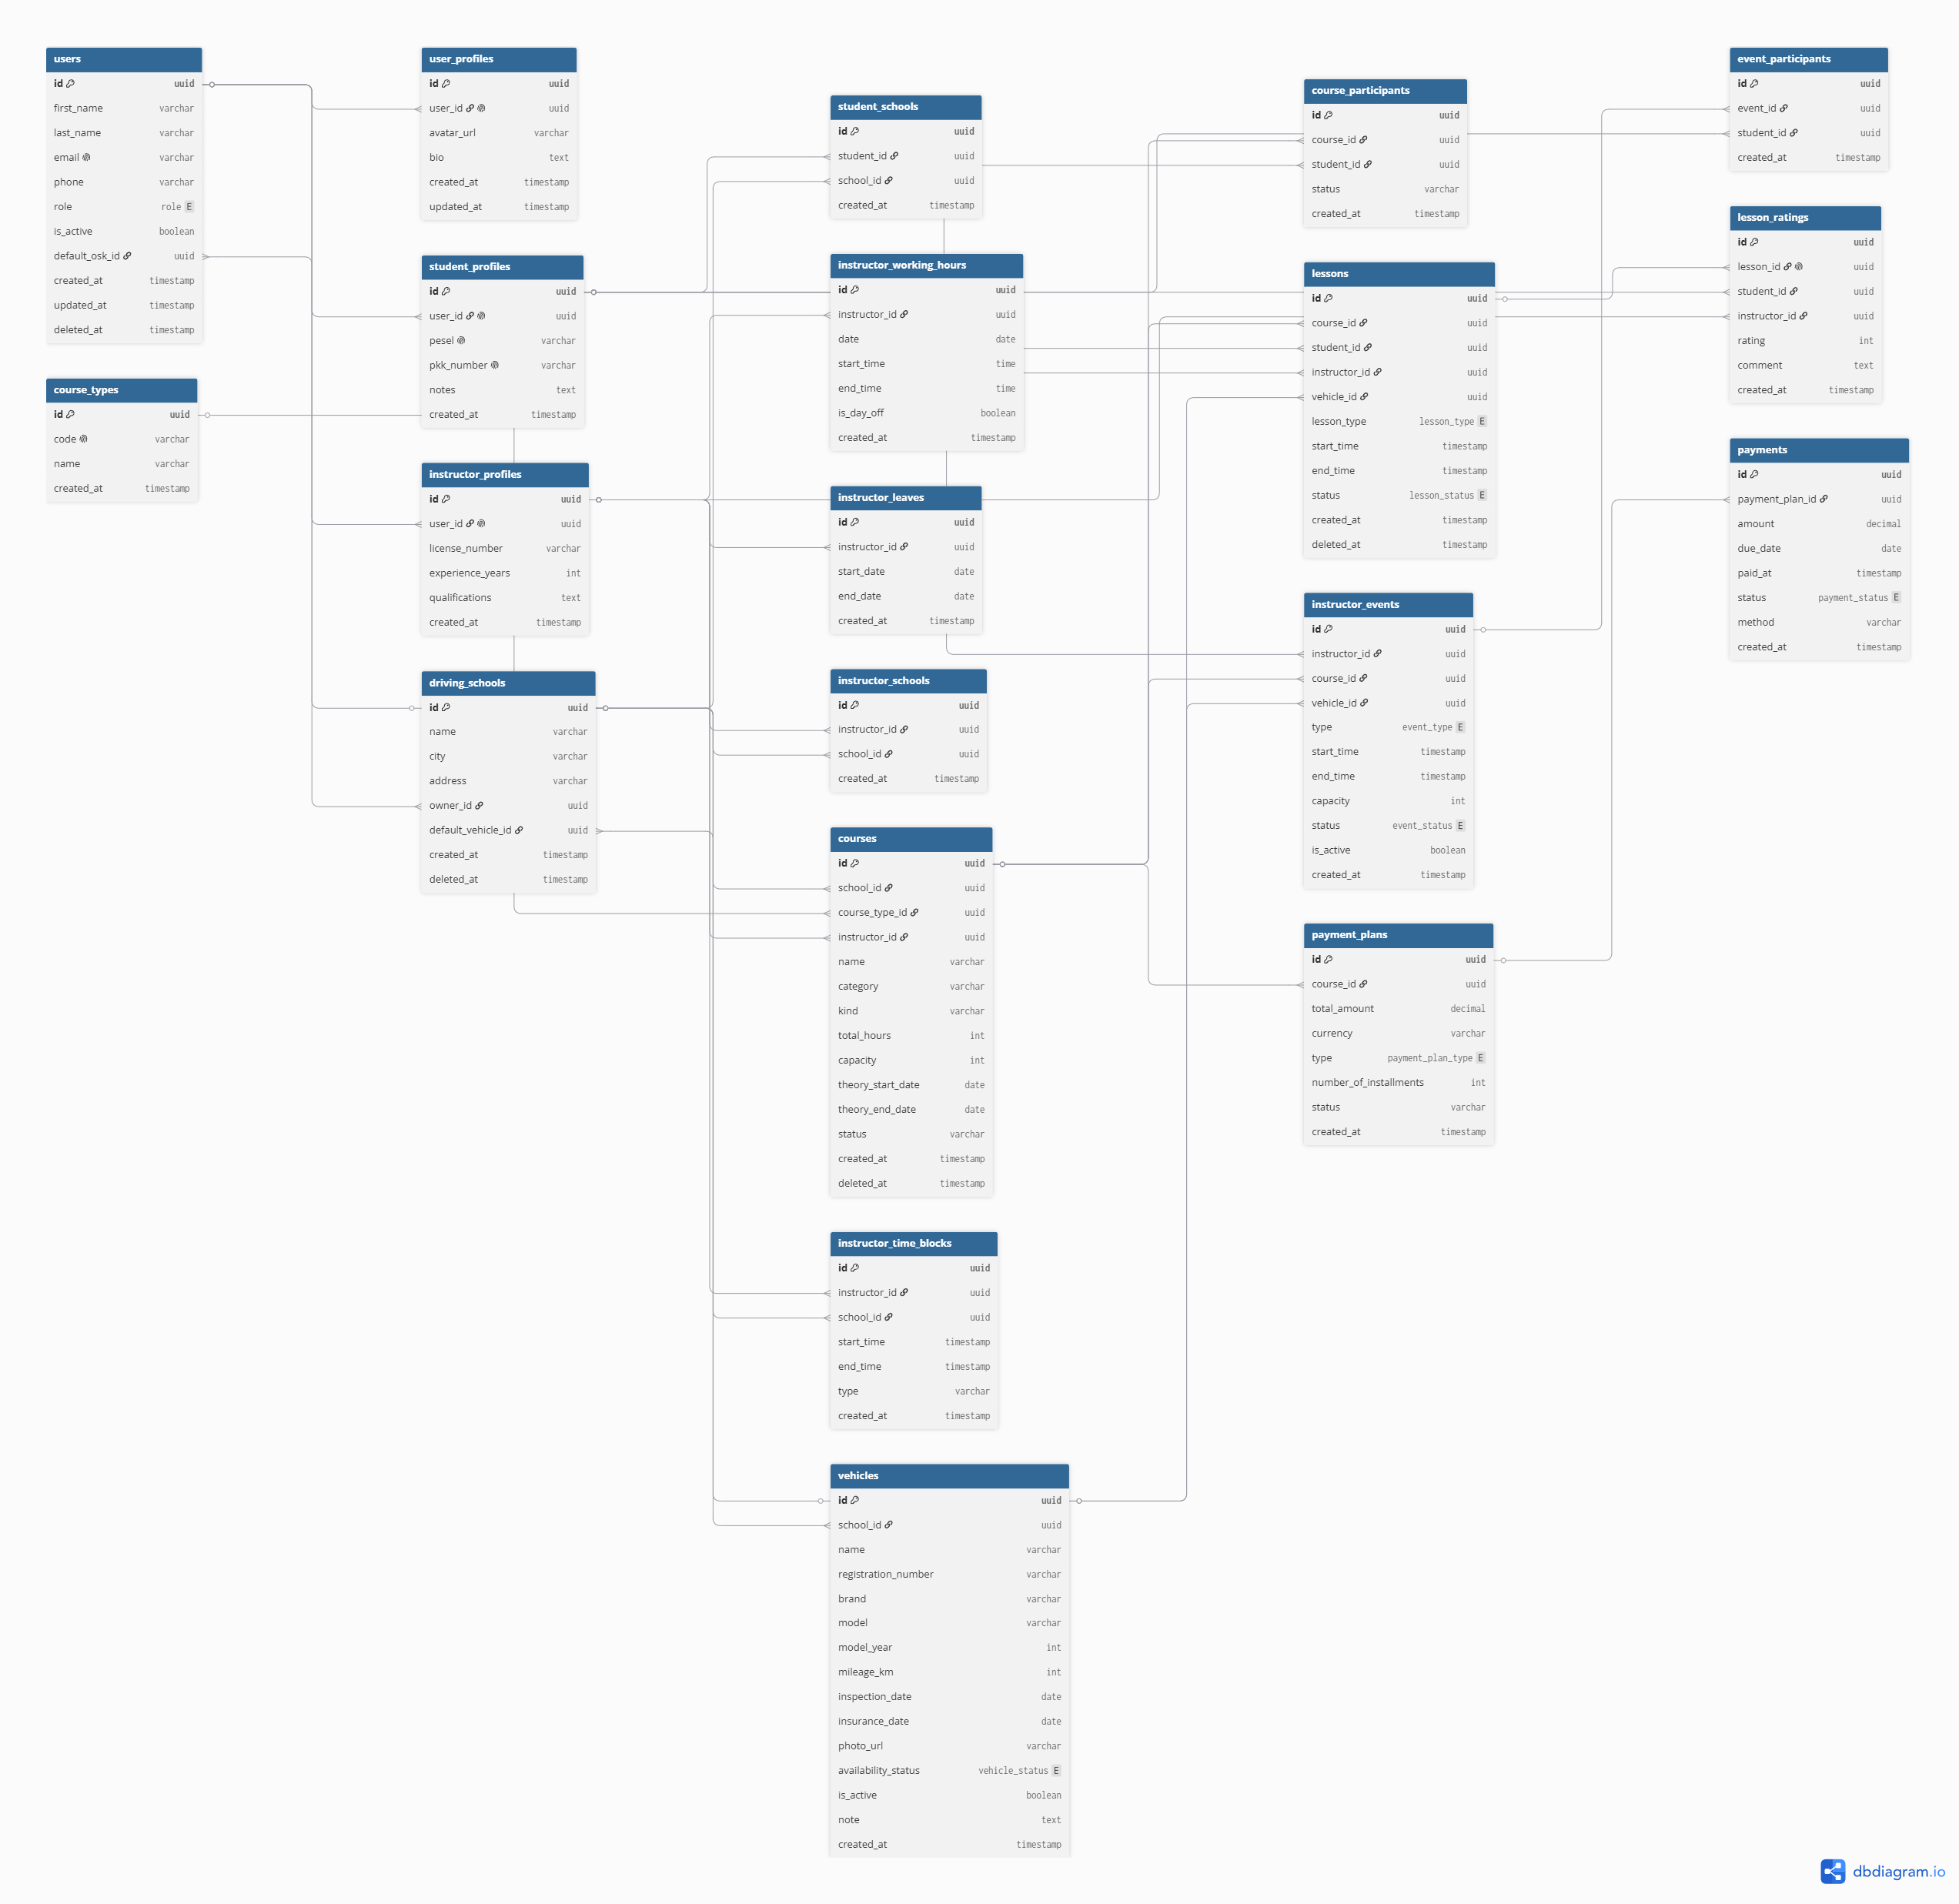
\includegraphics[width=\textwidth,height=0.76\textheight,keepaspectratio]{figures/generated/erd.png}
\caption{Diagram ERD bazy danych systemu OSK-Manager}
\label{fig:diagram-erd-osk-manager}
\wsizsource{Opracowanie własne}
\end{figure}
\section{Integralność danych}
\label{sec:integralnosc-danych}

Model danych zawiera relacje i ograniczenia pomagające zachować spójność informacji. Przykładowo adres e-mail użytkownika jest unikalny, numer rejestracyjny pojazdu jest unikalny w ramach szkoły, a przypisanie kursanta do kursu nie powinno się powtarzać. W bazie występują także indeksy przyspieszające wyszukiwanie danych w harmonogramie, na przykład po instruktorze, pojeździe, kursancie i czasie rozpoczęcia lekcji.

Sama struktura bazy nie zastępuje logiki biznesowej. Dlatego część reguł jest realizowana w serwisach backendowych. Dotyczy to przede wszystkim sprawdzania kolizji terminów, zgodności kursanta, instruktora i pojazdu z tym samym OSK oraz zasad dotyczących oceniania lekcji.

\section{Diagram klas}
\label{sec:struktura-diagram-klas}

Diagram klas systemu został przedstawiony wcześniej w rozdziale dotyczącym modelowania systemu, na rysunku \ref{fig:diagram-klas-osk-manager}. W kontekście struktury systemu pełni on rolę uproszczonego widoku domeny i pokazuje najważniejsze klasy biznesowe: użytkownika, ośrodek szkolenia, kurs, lekcję, pojazd, dostępność instruktora oraz płatność.

Właściwy model implementacyjny jest bardziej szczegółowy niż uproszczony diagram klas. W kodzie i schemacie bazy danych znajdują się dodatkowe encje pomocnicze, takie jak profile użytkowników, ustawienia szkoły, uczestnicy kursów, wydarzenia instruktorskie, uczestnicy wydarzeń, plany płatności i oceny lekcji. Diagram klas w dokumentacji pokazuje więc główny obraz domeny, natomiast opis bazy danych rozszerza go o szczegóły implementacyjne.
